\section{Introduction}

Hardware system verification has been developed over a large amount of
years, but mostly with limited approaches. Most of works used model
checking to verify their target components, from processor
verification~\cite{ProcVerif1, ProcVerif2} to cluster
verification~\cite{ClusterVerif}, which is the recent work. In order
to use model checking technique, one must first finitize the
state-space for exhaustive exploration, which naturally hinders
generalization. What should be defined and developed if one desires to
verify parametrized hardware system, such as complex pipelined
processors or multi-level cache-coherence protocols?

Defining formal hardware semantics is the very first step to answer
such question. In model checking it is not required to define
semantics for general hardware system, since checkers have their own
specific targets. However, in order to deal with all aspects of
hardware system, one should define semantics which can describe all
system behaviors. Finally, when formal semantics and verifications are
correctly attached to Hardware Description Languages (HDLs), we can
claim that real hardware components are verified.

Now the focus is moved to the semantics design: what is good semantics
for hardware system? First of all it should be intuitively
understandable, which implies that the semantics should logically
simulate system behaviors. Moreover, if it is employed for
verification, it should also be consistent with various proof aspects.

In this proposal, I propose to introduce a number of hardware
semantics, and to compare their pros and cons for better
understanding. I also propose to give formal consistency proofs for
those semantics, which prove that the semantics are convertible to
each other. All definitions and proofs will be formally given using
Coq theorem-proving system.

\section{Background: Guarded Atomic Action}\label{sec:background}
Traditional Register-Transfer Level (RTL) designs require hardware
designers to consider scheduling for all resources. During hardware
design, one has to ensure that any resource elements are correctly
employed, e.g., one should not write a register more than once in a
same cycle, which causes incorrect assignment. If a particular input
port of a hardware component is used more than once, we do not have
any guarantees for the output value, also causing incorrect use of
values. A well-known RTL design framework, Verilog, let users take
responsibility of this, thus one should carefully investigate if there
is an assignment which makes incorrect state transition.
%% This low-level approach, however, gives user a chance to directly
%% determine which values should be written in a cycle, therefore to
%% build a well-optimized hardware.
\begin{figure}[h]
  \centering
  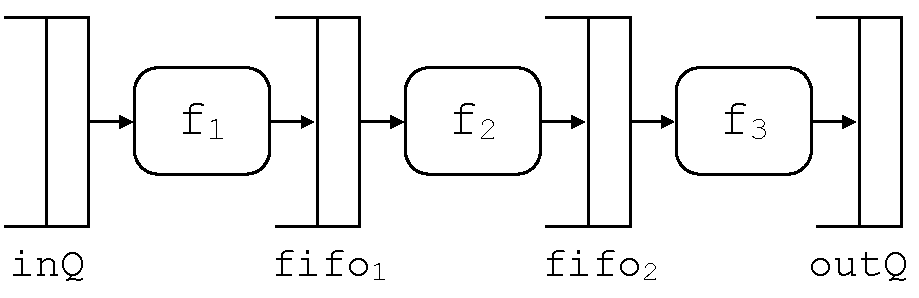
\includegraphics[width=0.5\textwidth]{figures/pipeline.pdf}
  \caption{A pipelined system}
  \label{fig:pipeline}
\end{figure}

A disadvantage of this approach is that having no separation between
functional parts and scheduling logic makes maintenance
harder. Consider a pipelined system where three systems $f_0$, $f_1$,
and $f_2$ are connected by fifos, as shown in
Fig.~\ref{fig:pipeline}. For simplicity, suppose that only one element
can reside in a fifo. Since there is only one element in a fifo, push
and pop cannot be requested in a same cycle -- it will cause
double-write. Now the problem occurs because we have no information
whether push and pop will be requested simultaneously or not. Thus in
this case, we cannot avoid an implementation tightly coupled with
scheduling logic; for each case of push and pop, there is no way for
user but to define different implementations. The design process
entangled with scheduling logic also makes verification harder. We
first have more cases to verify, as there will be different functional
parts as much as scheduling cases. We also have to determine whether
it is caused by funcaional parts or scheduling logic if there is an
error.

Guarded atomic action~\cite{GAA} is a design paradigm for correct and
effective scheduling as well as making up shortcomings of the RTL
designs. It is different from the traditional RTL designs mentioned
above. The main idea is that any hardware system has a (structural)
state component that can be captured by a set of variables that
represent registers or storage. State transition is done by a set of
rules, where a rule is a series of actions on this state. These
actions should be atomic -- an execution of an action should be
guaranteed to make a state transition purely caused by the action.
%% An atomic action induce a guard, a predicate to execute the
%% action. Guards are interpreted by a scheduler to generate a correct
%% schedule, which will be explained in the next section.

\section{Research Questions}

\subsection{Hardware Description Syntax}

\newcommand{\Mod}{\ensuremath{M}}
\newcommand{\ModC}[3]{\ensuremath{(#1, #2, #3)}}
\newcommand{\ModP}{\ensuremath{+}}

Before defining various hardware semantics, we first define a hardware
description language syntax, which will be the common basis for
defining semantics. First, a basic module $\Mod{} =
\ModC{s}{\vec{r}}{\vec{m}}$ can be composed of (internal) state $s$,
rules $\vec{r}$, and methods $\vec{m}$. Each rule or method is a
series of actions, explained in Section~\ref{sec:background}, which
only affects the internal state. Rules are fired by a scheduler which
controls the entire system. Methods can be called by some other
modules. Once modules are defined, now we can combine two modules to
build a combined module, using \ModP{} operator. Following is the
inductive definition of a module:

$$\begin{array}{rcl}
  \Mod{} & := & \ModC{s}{\vec{r}}{\vec{m}} \\
  & | & \Mod{} \ModP{} \Mod{} \\
\end{array}$$

One might raise several issues with this syntax definition. For
example, it can be asked whether rule/method names are globally unique
among all modules. This kind of question is interesting in that we can
give several solutions for it. We can globally check whether name
conflict occurs on a module syntax. Instead of this, we can always do
$\alpha$-conversion for all names in modules before two modules are
combined.

Once all syntactic issues are resolved, the next step is to give the
meaning of module. It requires to give the meaning of rule/method
execution and \ModP{} operator. Each semantics should have its own
meaning of these ingredients, which includes an ability to confirm
valid execution cases and to reject invalid ones.

\subsection{Modular Semantics Inspired by Labeled Transition System}

\subsection{Inlined Semantics}

\subsection{Small-step and Denotational Semantics}

\subsection{Semantic Consistency}

\section{Work Plan}

Ipsum

\section{References}

Ipsum
